% -*- TeX-master: "../all_the_notes.tex" -*-
\newpage
\section{4JJ-series Flux Qubit \cite{qui2016}}
\begin{framed}\noindent
  This   qubit   behaves  like   a   3JJ   qubit,  albeit   with   some
  \red{differences}:
  \begin{itemize}
  \item Can be operated in the single or double potential well regime;
  \item \red{Has a lower flux sensitivity and thus better to tune};
  \item      \red{Under       certain      conditions      \textbf{only
        \iket{1}\ilra\iket{2}}   allowed.   In   other  systems   other
      transitions are also possible} - no state leakage to \iket{3}.
  \end{itemize}
\end{framed}

\noindent
\subsection{Derivation of the Hamiltonian}
It's a load of bloat including:
\begin{enumerate}
\item Using phase loop quantisation
  \begin{equation}
    \varphi_1 + \varphi_2 + \varphi_\alpha + \varphi_\beta + 2\pi f_\text{tot} = 0;
  \end{equation}
\item    Kinetic    energy     evaluation,    using    emf    induction
  $ V = \dot{\Phi} $:
  \begin{equation}
    \begin{aligned}
      \mathcal{T} = & \frac{1}{2}\sum C_iV_i^2\\
      &                                                               =
      \frac{C}{2}\left(\frac{\Phi_0}{2\pi}\right)^2\left\lbrace\dot{\varphi}^2_1
        +    \dot{\varphi}^2_2    +   \alpha\dot{\varphi}^2_\alpha    +
        \beta\left[\dot{\varphi}_1       +      \dot{\varphi}_2       +
          \dot{\varphi}_\alpha                  +                  2\pi
          \dot{f}_\text{tot}\right]^2\right\rbrace;
    \end{aligned}
  \end{equation}
\item Potential energy
  \begin{equation}
    U = \sum E_{Ji}\left[1 - \cos(\varphi_i)\right].
  \end{equation}
\item Inductive energy
  \begin{equation}
    U_L = \frac{\Phi_0^2}{2L}\left(f_\text{tot} - f_\text{ext}\right)^2.
  \end{equation}
\item      Some      complicated     transformation      that      maps
  $  \varphi_1, \varphi_2,  \varphi_\alpha  \ira \varphi_+,  \varphi_-,
  \varphi, \xi $, where
  \begin{equation}
    \xi = f_\text{tot} - f_e \approx f_a(t)\ (\text{negligible flux linxed by current}),
  \end{equation}
  \begin{figure}[h]
    \centering 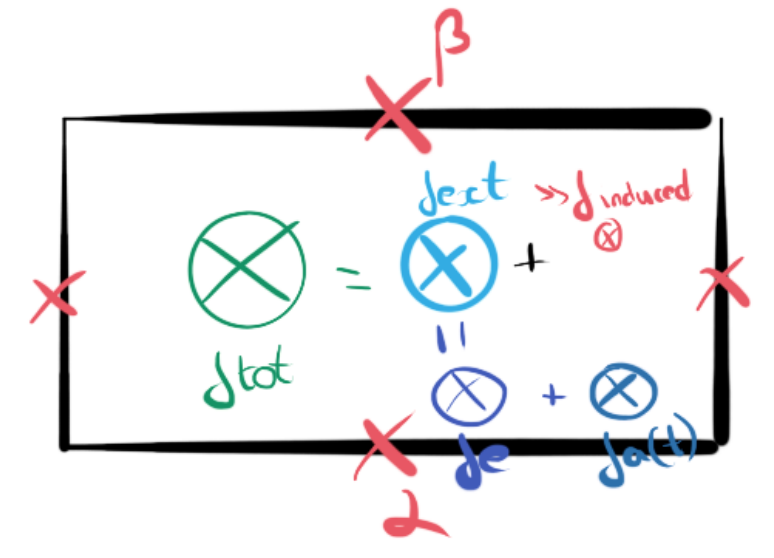
\includegraphics[height=5cm]{flux4jj_1}
  \end{figure}

  \noindent
  \noindent is  the time dependent  component of the magnetic  field to
  arrive at the largrangian
  \begin{equation}
    \begin{aligned}
      \mathcal{L} & = \mathcal{T} - U\\
      & =  \frac{C}{2}\left(\frac{\Phi_0}{2\pi}\right)^2\left(\dot{\varphi}^2 + \Gamma_+\dot{\varphi}_+^2 + \Gamma_-\dot{\varphi}_-^2 + \Gamma_\xi\xi^2\right)\\
      &     -     U(\varphi,     \varphi_+,     \varphi_-,     \xi)     -
      \frac{\Phi_0^2}{2L}\left(\xi - f_\text{a}\right)^2
    \end{aligned}
  \end{equation}
\item Finding the canonical momenta
  \begin{equation}
    P_i = \frac{d\mathcal{L}}{d\varphi_i}
  \end{equation}

  \noindent        and        evaluating        the        Hamiltonian,
  $ \mathcal{H} = \sum P_i\varphi_i - \mathcal{L} $.
\item Splitting the Hamiltonian up into a Harmonic oscillator part
  \begin{equation}
    \mathcal{H} = 4E_C\left(P^2 + \frac{P_+^2}{\Gamma_+} + \frac{P_-^2}{\Gamma_-}\right) + U(\varphi, \varphi_+, \varphi_-, \xi) + \red{\mathcal{H}_\text{osc}},
  \end{equation}

  \noindent \red{which is always in the ground state, due to its energy
    being much  higher than the qubit  levels.  Thus it can  be dropped
    from consideration.}
\end{enumerate}

\subsection{Bloat over}
So now lets have a look at some implications of this Hamiltonian.

\begin{enumerate}
\item\
  \begin{framed}\noindent
    \textbf{The potential  landscape that forms} has  adjustable single
    and double wells through the 0.5 threshold in 3 JJ qubit.
  \end{framed}

\begin{figure}[h]
  \centering 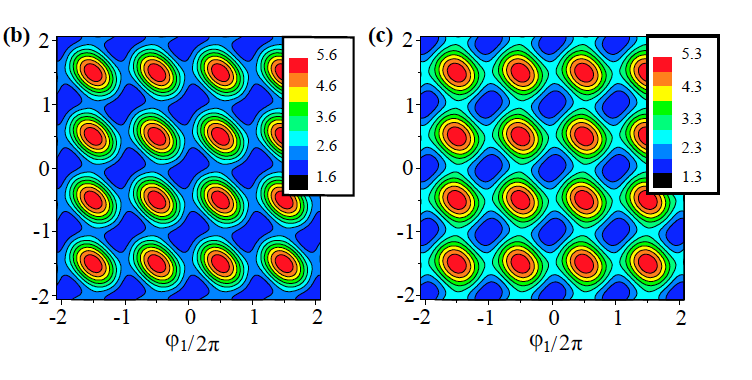
\includegraphics[height=6cm]{flux4jj_2}
\end{figure}

\noindent
\item                  The                 solution                  of
  $ \mathcal{H}_0\psi(\mathbf{\varphi})  = E\psi(\mathbf{\varphi}) $ is  looked for
  in a block wave form
  \begin{equation}
    \Psi(\mathbf{\varphi}) = u(\mathbf{\varphi}) = \sum_{\mathbf{K}}a_\mathbf{K}e^{i\mathbf{K}.\mathbf{\varphi}}.
  \end{equation}

\item    In   the    single   well    configuration   (\textbf{bottom},
  $ \beta < 0.3 $) the bands are flatter and less susceptible to flux noise
  than in the double well (\textbf{top}, $ \beta > 0.3 $) case.

\begin{figure}[h]
  \centering 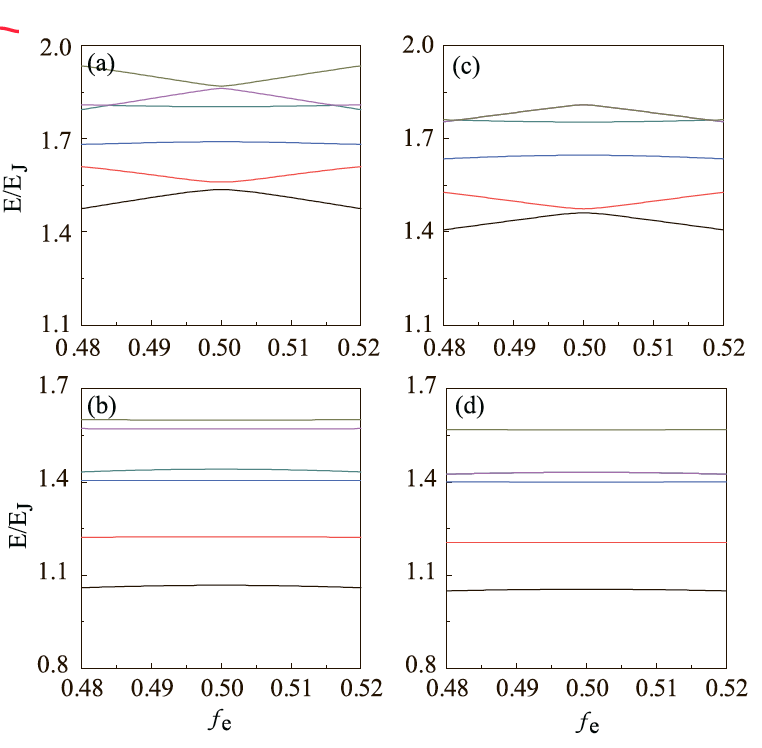
\includegraphics[height=7cm]{flux4jj_3}
\end{figure}

\noindent
\begin{framed}\noindent
  Note the superior separation of the levels in both the 3JJ
\end{framed}

\begin{framed}\noindent
  \red{\textbf{The  addition  of a  time  dependent  field changes  the
      hamitlonian to give a perturbation}}:
  \begin{equation}
    \begin{aligned}
      \mathcal{H} & = \mathcal{H}_0 - I\Phi_a(t)\\
      & I = \text{ effective current, which is a monster of an equation}\\
      & \Phi_a(t) = \iabs{\Phi_a}\cos(\omega_at).
    \end{aligned}
  \end{equation}

  \noindent  and we  have a  transition  that is  calculated using  the
  eigenstates of the original Hamiltonian

  \begin{equation}
    t_{ij} = \bra{i}I\Phi_a\ket{j}.
  \end{equation}
\end{framed}

\item The results are:
  \begin{itemize}
  \item At  the degeneracy  point, \iket{1}\ilra\iket{3}  is forbidden,
    and we have a $ \Xi $ energy ladder.  Everywhere else it's a $ \Delta $
    \begin{figure}[h]
      \centering 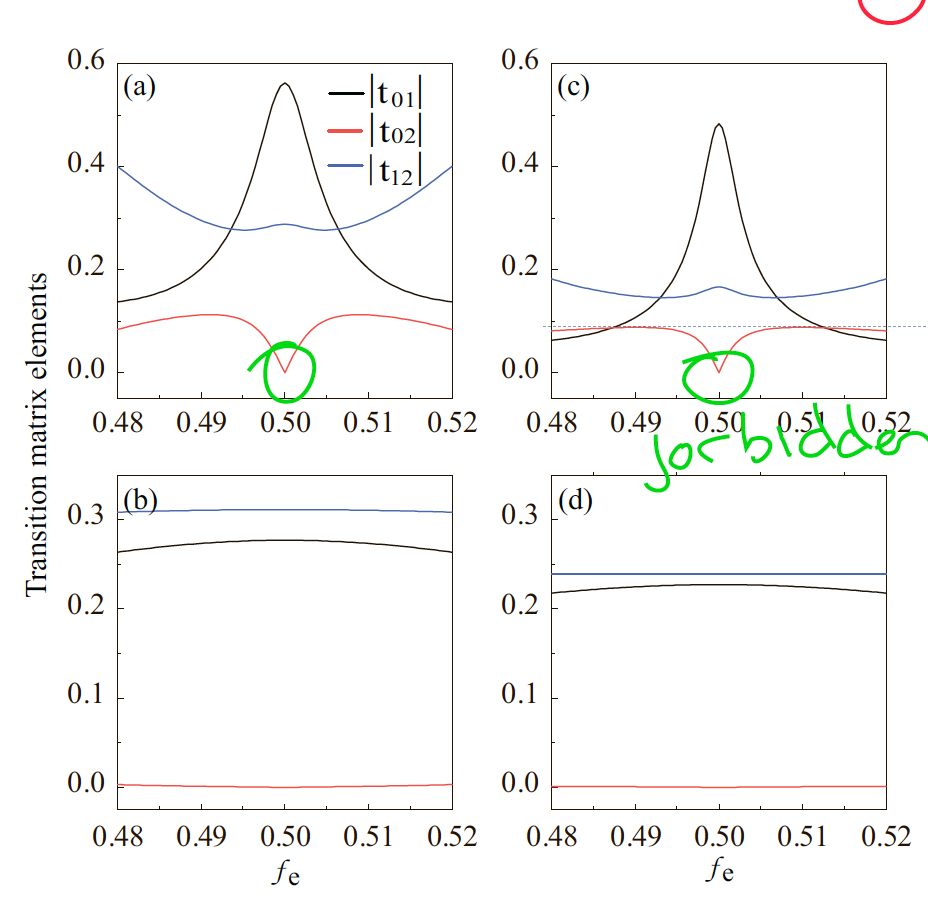
\includegraphics[height=6cm]{flux4jj_4}
    \end{figure}

    \noindent
  \item  For   low  $  \beta   $  all  transitions  are   supressed  except
    \iket{1}\ilra\iket{2}.   \textbf{This  makes  it  a  perfect  qubit
      system, with no leakage to other energy levels.}

    \begin{figure}[h]
      \centering 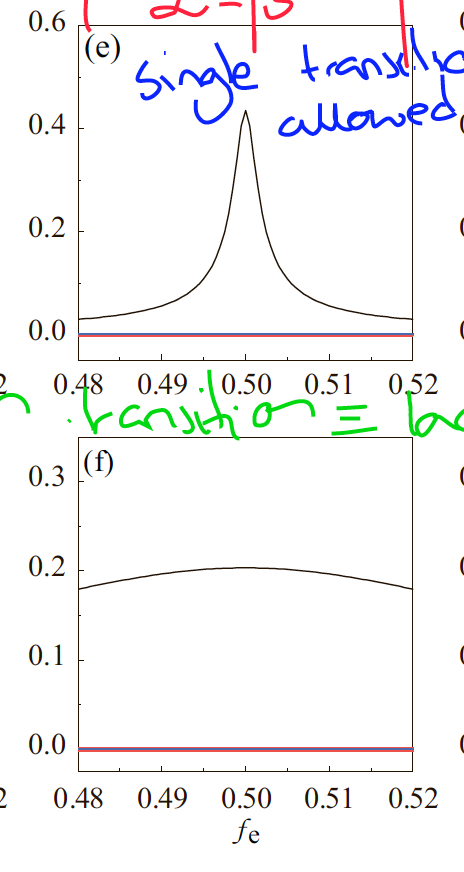
\includegraphics[height=6cm]{flux4jj_5}
    \end{figure}

  \end{itemize}
\end{enumerate}
